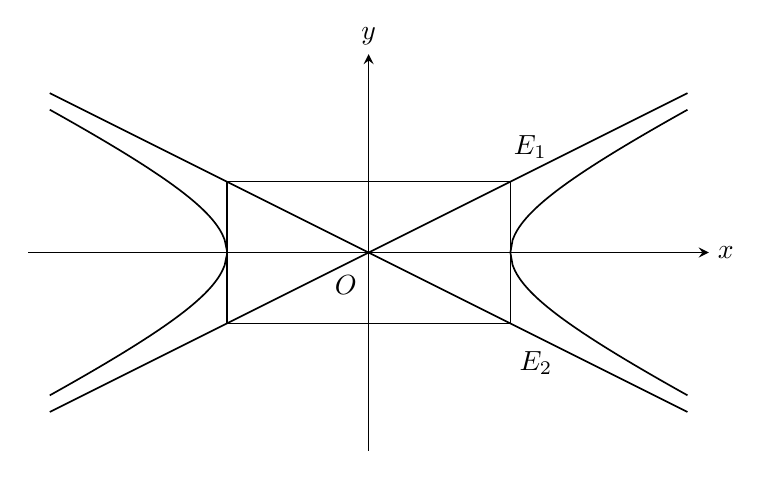
\begin{tikzpicture}[x=0.9cm,y=0.9cm,line width=.6pt,>=stealth,font=\normalsize]
\draw[->] (-4.8,0)--(4.8,0) node[right,xshift=3.0pt,inner sep=0pt] {$x$};
\draw[->] (0,-2.8)--(0,2.8) node[above,yshift=3.0pt,inner sep=0pt] {$y$};
\node[below left,xshift=-4pt,yshift=-8pt,inner sep=0pt] at (0,0) {$O$};
\draw[solid,domain=-4.5:4.5,samples=120] plot (\x,{\x/2});
\draw[solid,domain=-4.5:4.5,samples=120] plot (\x,{-\x/2});
\draw[solid] (-2,1)--(2,1)--(2,-1)--(-2,-1)--cycle;
\draw[solid,domain=2:4.5,samples=80] plot (\x,{sqrt(\x*\x/4-1)});
\draw[solid,domain=2:4.5,samples=80] plot (\x,{-sqrt(\x*\x/4-1)});
\draw[solid,domain=-4.5:-2,samples=80] plot (\x,{sqrt(\x*\x/4-1)});
\draw[solid,domain=-4.5:-2,samples=80] plot (\x,{-sqrt(\x*\x/4-1)});
\node[above right,xshift=-1pt,yshift=6pt,inner sep=2pt] at (2,1) {$E_{1}$};
\node[below right,xshift=1pt,yshift=-8pt,inner sep=2pt] at (2,-1) {$E_{2}$};
\end{tikzpicture}
